\documentclass[a4paper, 12pt]{article}
\usepackage[utf8]{inputenc}
\usepackage[T1]{fontenc}
\usepackage[ngerman]{babel}
\usepackage{geometry}
\usepackage{listings}
\usepackage{xcolor}
\usepackage{hyperref}
\usepackage{helvet}
\usepackage{titlesec}
\usepackage{setspace}
\usepackage{graphicx}
\usepackage{pdfpages}
\usepackage{fancyhdr}
\usepackage{float}
\usepackage{enumitem}
\usepackage{tikz}
\usepackage{etoolbox}


\lstdefinelanguage{JavaScript}{
    keywords={break, case, catch, continue, debugger, default, delete, do, else, finally, for, function, if, in, instanceof, new, return, switch, this, throw, try, typeof, var, void, while, with},
    keywordstyle=\color{blue}\bfseries,
    ndkeywords={class, const, enum, export, extends, import, super, implements, interface, let, package, private, protected, public, static, yield, null, true, false},
    ndkeywordstyle=\color{darkgray}\bfseries,
    identifierstyle=\color{black},
    sensitive=false,
    comment=[l]{//},
    morecomment=[s]{/*}{*/},
    commentstyle=\color{purple}\ttfamily,
    stringstyle=\color{red}\ttfamily,
    morestring=[b]',
    morestring=[b]"
}

\lstset{
    language=JavaScript,
    extendedchars=true,
    basicstyle=\footnotesize\ttfamily,
    showstringspaces=false,
    showspaces=false,
    numbers=left,
    numberstyle=\footnotesize,
    numbersep=9pt,
    tabsize=2,
    breaklines=true,
    showtabs=false,
    captionpos=b
}
\geometry{a4paper, left=2.5cm, right=2.5cm, top=3cm, bottom=3cm, headsep=1.5cm}

\setlength{\parindent}{0pt}
\setlength{\parskip}{6pt}
\graphicspath{ {./images/} }

\pagestyle{fancy}
\fancyhf{}
\rhead{\vspace{0.2cm}
\includegraphics[width=4cm]{hs_mainz_logo}}
\fancypagestyle{plain}{
    \fancyhf{}
    \rhead{\vspace{0.2cm}
\includegraphics[width=4cm]{hs_mainz_logo}}
}
\renewcommand{\headrulewidth}{0pt}
\renewcommand{\footrulewidth}{0pt}
\fancyfoot[C]{\thepage}

\newcounter{lastroman}
\newrobustcmd{\switchtopage}[1]{
    \clearpage
    \setcounter{lastroman}{\value{page}}
    \pagenumbering{#1}
}
\newrobustcmd{\switchback}{
    \clearpage
    \pagenumbering{Roman}
    \setcounter{page}{\value{lastroman}}
}

% Document
\begin{document}

    \pagenumbering{Roman}

    \begin{titlepage}
    \centering
    \vspace*{1cm}

    
\includegraphics[width=0.4\textwidth]{hs_mainz_logo}\\
    \vspace{1.5cm}

    \textbf{\LARGE Praxismodul I}\\
    \vspace{0.5cm}
    \textbf{\Large Collectiqo}\\
    \vspace{1.5cm}

    \textbf{Hochschule Mainz}\\
    \vspace{0.5cm}
    Fachbereich Wirtschaft\\
    \vspace{0.5cm}
    B.Sc. Wirtschaftsinformatik dual\\
    \vspace{1.5cm}

    \textbf{Authors:}\\
    Bindernagel, Lorenz\\
    Schäfer, Robin\\
    Šimić, Darko\\
    Struve, Anika\\
    \vfill

    \today
\end{titlepage}

    \newpage

    \setcounter{page}{2}
    \tableofcontents
    \newpage

    \switchtopage{arabic}

    \subsection{Motivation}\label{subsec:Motivation}


Das Sammeln von Kulturgütern ist ein Bedürfnis von vielen verschiedenen Menschen und eine Praxis, die Einblicke in Geschichte, Identität und ästhetische Vorlieben gewährt.
Es ist eine Leidenschaft, die Menschen verschiedener Hintergründe und Interessen verbindet, sei es das Sammeln von Parfumflaschen, Videospielen oder historischen Münzen.
Das Projektteam dient hierbei als Beispiel, da jedes Mitglied mindestens eine Sammlerleidenschaft verfolgt.
Bei mehreren Sammlungen, die man pflegt, fällt jedoch ein erhöhter Pflegeaufwand auf. \par
Trotz des reichen Angebots an Online-Plattformen zur Verwaltung einzelner Sammlungen fehlt bisher eine universelle Plattform, die es ermöglicht, mehrere Sammlungen unterschiedlicher Güter einheitlich zu digitalisieren. \par
Daher ist es das Ziel dieses Praxisprojektes, eine entsprechende Webseite aufzubauen, welche für Sammlungen jeglicher Art sowohl vorgefertigte als auch anpassbare Vorlagen bietet, mit denen diese organisiert, dokumentiert und auch präsentiert werden können.
Dies würde den Pflegeaufwand für Sammler verringern und spricht im großen Interesse des Projektteams.


\subsection{Marktanalyse / Technologische Grundlagen}\label{subsec:Marktanalyse-TechnologischeGrundlagen}

Um Anforderungen an das Projekt zu definieren und die Plattform bestmöglich zu differenzieren, wurde zwecks diesem eine Marktanalyse zu Sammlerplattformen betrieben.
Hierbei wurden auf Aspekte wie die Zielgruppe, das Angebot auf dem Markt und einzelner Plattformen, die Benutzerfreundlichkeit und aktuelle Markttrends geachtet. \par
Die Zielgruppe bezieht sich, wie in KAPITEL 1-1 beschrieben, auf Sammler verschiedener Sachgüter. \linebreak


Das Angebot der Plattformen unterscheidet sich in ihrer Spezialität und ihrer Zielrichtung.
Zwei der ausgewerteten Webseiten bieten für unterschiedliche Sammelgüter die Dokumentierung, Präsentation und Kapitalisierung von Sammelgütern an.
Restliche Webseiten bieten speziell für eine Kategorie von Sammlerobjekten dieselben Funktionen.
Keine Webseite bietet die Eigenerstellung einer Sammlung beziehungsweise Kategorie an. \par

Die Benutzerfreundlichkeit ist ein wichtiger Faktor für den Erfolg von Sammlerplattformen.
Eine intuitive Benutzeroberfläche, ein ansprechendes UI-Design, klare Kategorisierung der Sammelgüter und einfache Such- und Filterfunktionen tragen dazu bei, dass Benutzer gerne die Plattform benutzen.
Hierbei waren etwa die Hälfte der untersuchten Webseiten subjektiv gut gestaltet und erfüllen die genannten Anforderungen, die restlichen Seiten schienen im Design veraltet oder unhandhablich. \par

In den letzten Jahren hat die Nachfrage nach Sammlerobjekten zugenommen, sowohl von traditionellen Sammlern als auch von neuen Zielgruppen, die das Potenzial von Sammlerstücken als Investition erkannt haben.
Die Popularität von Online-Marktplätzen, wie beispielsweise eBay, hat ebenfalls dazu beigetragen, den Sammlermarkt zu beleben und den Zugang zu seltenen und einzigartigen Stücken zu erleichtern. \par
Insgesamt ist der Markt für Sammlerplattformen lebendig und vielfältig, jedoch nicht individualisierbar für Nischensammlungen. \par
Da die Analyse anhand der vorhandenen Daten verschiedener Plattformen betrieben wurde und keine Quellen bezüglich Personenbefragungen gefunden wurden, wurde eine anonyme Umfrage erstellt, in der Personen befragt wurden, ob sie Sammeln, wie Sie ihre Kollektion handhaben, und ob diese Interesse an einer benutzerfreundlichen Universalplattform zeigen. \linebreak

(Umfrageergebnisse \& für Analyse Quellen und Grafiken incoming)


    \newpage

    \subsection{Zieldefinition}\label{subsec:Zieldefinition}
Das Ziel dieses Projekts ist die Entwicklung und Implementierung einer universellen Sammlerplattform, die es Benutzern ermöglicht, ihre Sammlungen digital zu verwalten, zu präsentieren und mit anderen zu teilen.
Diese Plattform soll benutzerfreundlich, flexibel und skalierbar sein, um eine breite Palette von Sammlerbedürfnissen abzudecken.

% Wir könnten hier sicherlich auch das Wording Meilensteine nutzen, finde ich besser als Teilergebnisse
\subsection{Teilergebnisse}\label{subsec:Teilergebnisses}
Die Teilergebnisse lassen sich aus dem Konzept in ~\ref{subsec:Designphase} ableiten.
Grundlegende Teilergebnisse sind die Erstellung des Frontends, die Erstellung des Backends und die Einrichtung einer Datenbank.
Neben diesen Zielen, die sich aus der verwendeten Architektur ergeben, ist ein weiteres Teilergebnis das Hosting der Website und der Datenbank.
Für jedes Teilergebnis sind Voranalysen notwendig, da die Programmierung einer Webanwendung für das gesamte Team neu ist.
Als Ausgangspunkt für die Analyse diente GitHub Eduction, das mit dem Kurs Intro to Web Development einige Tools für die Entwicklung von Websites zur Verfügung stellt.
Die in der Analyse ausgewählten Tools sind in ~\ref{subsec:Tools} aufgelistet.

Die Teilergebnisse sind eng miteinander verknüpft.
Das Hosting der Website und der Datenbank sind von entscheidender Bedeutung.
Insbesondere das Backend ist ohne die Datenbank nur schwer zu entwickeln.
Das Hosting der Website ist wichtig, um die integrierten Funktionen direkt live testen zu können.
Die Entwicklung von Frontend, Backend und Datenbank ist eng miteinander verzahnt.
Frontend und Datenbank lassen sich separat einrichten, das Backend ist für die Kommunikation der beiden Bereiche unerlässlich.
Während die drei Bereiche einzelne Teilergebnisse darstellen, erfolgt der Großteil der Programmierung parallel.

Das Frontend ist alles, womit der Benutzer letztendlich auf der Website interagieren kann.
Beispiele hierfür sind die Login-Seite, die Ansicht der verschiedenen Sammlungen und die Seite zur Erstellung von Vorlagen.
Im Anhang finden sich Mockups, die während des anfänglichen Brainstormings der Projektidee entstanden sind.
Das Backend ist für die Kommunikation zwischen dem Frontend und der Datenbank verantwortlich.
Es soll die Daten aus der Datenbank an das Frontend zur Anzeige weiterleiten.
Außerdem soll es Änderungen an den Daten, die in der Benutzeroberfläche vorgenommen werden, an die Datenbank kommunizieren.
Dabei ist es wichtig, dass die Funktionen sicherstellen, dass die Datenbank dynamisch auf Basis der Benutzereingaben skaliert wird.
Die Logik der Website sollte in diesem Teil des Programms definiert werden.
Das Datenbanksystem ist der Ort, an dem Informationen über Benutzer und Sammlungen gespeichert werden.
Die Datenbankform der Sammlungsvorlagen wird hier gespeichert.
Es muss so konfiguriert sein, dass das dynamische Hinzufügen und Löschen ganzer Tabellen möglich ist.
% Vllt mal ein Mockup für ein Template erstellen

\subsection{Definitions of done}\label{subsec:DoD}
Im Rahmen des Projekts wurden die folgenden Definitions of Done festgelegt, um den erfolgreichen Abschluss der verschiedenen Projektaufgaben und -phasen sicherzustellen:

\begin{enumerate}
    \item \textbf{Die Idee des Projektes ist erstellt:}
    \begin{itemize}[label=--, itemsep=0pt, parsep=0pt]
        \item Eine klare und detaillierte Beschreibung des Projektziels und der Motivation liegt vor.
        \item Das Projektziel ist verständlich und umfassend dokumentiert.
    \end{itemize}

    \item \textbf{Auswahl der genutzten Software- bzw. Projektwerkzeuge ist erfolgt:}
    \begin{itemize}[label=--, itemsep=0pt, parsep=0pt]
        \item Alle notwendigen Software- und Projektmanagement-Tools sind ausgewählt und dokumentiert.
        \item Die Gründe für die Auswahl der jeweiligen Werkzeuge sind festgehalten.
    \end{itemize}

    \item \textbf{Projektplanung ist angelegt:}
    \begin{itemize}[label=--, itemsep=0pt, parsep=0pt]
        \item Ein detaillierter Projektplan mit Zeitplan, Meilensteinen und Ressourcenplanung ist erstellt.
        \item Der Projektplan ist mit dem Projektteam abgestimmt und genehmigt.
    \end{itemize}

    \item \textbf{Erstellung von Konzept und Projektplan (Abgabe 1) erfolgreich und genehmigt:}
    \begin{itemize}[label=--, itemsep=0pt, parsep=0pt]
        \item Das Konzept und der Projektplan sind fertiggestellt und den entsprechenden Gremien oder Betreuern vorgelegt.
        \item Eine formelle Genehmigung oder Freigabe wurde erteilt.
    \end{itemize}

    \item \textbf{Anlegen der Projektumgebung mithilfe der Software- bzw. Projektwerkzeuge erfolgte:}
    \begin{itemize}[label=--, itemsep=0pt, parsep=0pt]
        \item Die Projektumgebung ist vollständig eingerichtet, einschließlich aller erforderlichen Software- und Hardwarekomponenten.
        \item Alle Teammitglieder haben Zugang und die notwendige Schulung für die genutzten Werkzeuge erhalten.
    \end{itemize}

    \item \textbf{Backend-System ist implementiert:}
    \begin{itemize}[label=--, itemsep=0pt, parsep=0pt]
        \item Das Backend-System ist vollständig entwickelt und funktionsfähig.
        \item Alle geplanten Funktionen und Schnittstellen sind implementiert und getestet.
    \end{itemize}

    \item \textbf{Frontend-System ist implementiert:}
    \begin{itemize}[label=--, itemsep=0pt, parsep=0pt]
        \item Das Frontend-System ist vollständig entwickelt und funktionsfähig.
        \item Das Design entspricht den vorher festgelegten Spezifikationen und ist benutzerfreundlich.
    \end{itemize}

    \item \textbf{Datenbanksystem ist implementiert:}
    \begin{itemize}[label=--, itemsep=0pt, parsep=0pt]
        \item Die Datenbank ist eingerichtet, strukturiert und alle notwendigen Tabellen und Beziehungen sind vorhanden.
        \item Die Datenbank erfüllt die Anforderungen hinsichtlich Performance und Sicherheit.
    \end{itemize}

    \item \textbf{Verknüpfung der drei Systeme erfolgte:}
    \begin{itemize}[label=--, itemsep=0pt, parsep=0pt]
        \item Backend, Frontend und Datenbanksystem sind nahtlos integriert.
        \item Die Kommunikation zwischen den Systemen ist getestet und funktioniert einwandfrei.
    \end{itemize}

    \item \textbf{Account-Erstellung und Benutzer-Login ist möglich:}
    \begin{itemize}[label=--, itemsep=0pt, parsep=0pt]
        \item Nutzer können erfolgreich Accounts erstellen und sich in das System einloggen.
        \item Die Authentifizierungsmechanismen sind sicher und funktionieren zuverlässig.
    \end{itemize}

    \item \textbf{Vorhandene „Sammlungen“-Templates können genutzt werden:}
    \begin{itemize}[label=--, itemsep=0pt, parsep=0pt]
        \item Standard-Templates für Sammlungen sind verfügbar und können von den Benutzern angewendet werden.
        \item Diese Templates sind funktional und ansprechend gestaltet.
    \end{itemize}

    \item \textbf{Benutzer kann erfolgreich eigene Templates anlegen:}
    \begin{itemize}[label=--, itemsep=0pt, parsep=0pt]
        \item Nutzer haben die Möglichkeit, eigene Templates für ihre Sammlungen zu erstellen und zu speichern.
        \item Die Anpassung und Nutzung dieser Templates ist intuitiv und problemlos möglich.
    \end{itemize}

    \item \textbf{Benutzerrechte-Einstellungen sind passend:}
    \begin{itemize}[label=--, itemsep=0pt, parsep=0pt]
        \item Benutzerrechte und -rollen sind definiert und korrekt implementiert.
        \item Die Plattform stellt sicher, dass Benutzer nur auf die ihnen zugewiesenen Bereiche und Funktionen zugreifen können.
    \end{itemize}

    \item \textbf{Alle notwendigen Tests erfolgreich:}
    \begin{itemize}[label=--, itemsep=0pt, parsep=0pt]
        \item Alle geplanten Tests (Unit-Tests, Integrationstests, Systemtests, Usability-Tests) sind abgeschlossen.
        \item Die Testergebnisse sind dokumentiert und alle kritischen Fehler sind behoben.
    \end{itemize}

    \item \textbf{Projektdokumentation ist erstellt:}
    \begin{itemize}[label=--, itemsep=0pt, parsep=0pt]
        \item Eine vollständige und detaillierte Dokumentation des Projekts ist vorhanden.
        \item Die Dokumentation umfasst alle Aspekte der Entwicklung, Implementierung und Nutzung der Plattform.
    \end{itemize}

    \item \textbf{Produktpräsentation fertiggestellt:}
    \begin{itemize}[label=--, itemsep=0pt, parsep=0pt]
        \item Eine umfassende Produktpräsentation ist vorbereitet, die alle wichtigen Funktionen und Vorteile der Plattform darstellt.
        \item Die Präsentation ist auf die Zielgruppe abgestimmt und beinhaltet anschauliche Beispiele und Demonstrationen.
    \end{itemize}

    \item \textbf{Projektbericht + Präsentation (Abgabe 2) erfolgreich und abgenommen:}
    \begin{itemize}[label=--, itemsep=0pt, parsep=0pt]
        \item Der abschließende Projektbericht ist fertiggestellt und eingereicht.
        \item Die Präsentation wurde erfolgreich durchgeführt und das Projekt wurde offiziell abgenommen.
    \end{itemize}
\end{enumerate}


\subsection{Projektstrukturplan}\label{subsec:PSP}
Lorenz ipsum dolor sit amet, consetetur sadipscing elitr, sed diam nonumy eirmod tempor invidunt ut labore et dolore magna aliquyam erat, sed diam voluptua.
At vero eos et accusam et justo duo dolores et ea rebum.
Stet clita kasd gubergren, no sea takimata sanctus est Lorem ipsum dolor sit amet.
Lorenz ipsum dolor sit amet, consetetur sadipscing elitr, sed diam nonumy eirmod tempor invidunt ut labore et dolore magna aliquyam erat, sed diam voluptua.
At vero eos et accusam et justo duo dolores et ea rebum.
Stet clita kasd gubergren, no sea takimata sanctus est Lorem ipsum dolor sit amet.
Lorenz ipsum dolor sit amet, consetetur sadipscing elitr, sed diam nonumy eirmod tempor invidunt ut labore et dolore magna aliquyam erat, sed diam voluptua.
At vero eos et accusam et justo duo dolores et ea rebum.
Stet clita kasd gubergren, no sea takimata sanctus est Lorem ipsum dolor sit amet.

\begin{figure}[H]
    \centering
    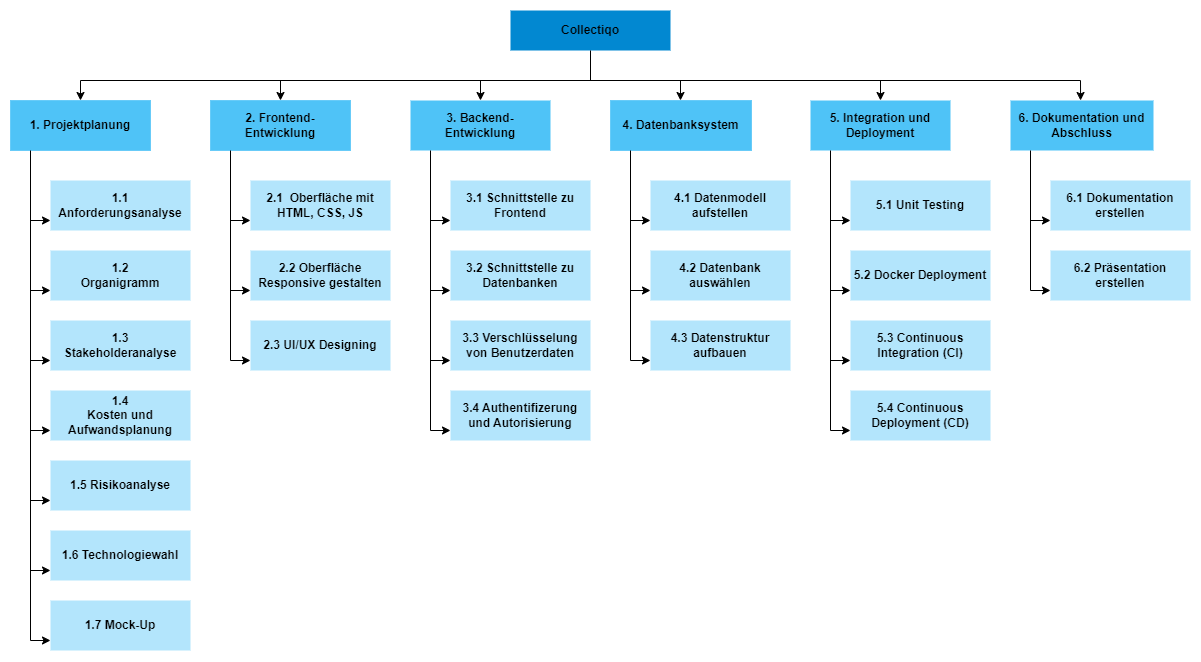
\includegraphics[width=1.0\textwidth]{psp}
    \caption{Projektstrukturplan}
\end{figure}
    \newpage

    \section{Projektmanagement}\label{sec:projektmanagement}

\subsection{Organigramm}\label{subsec:Organigramm}

\begin{figure}[H]
    \centering
    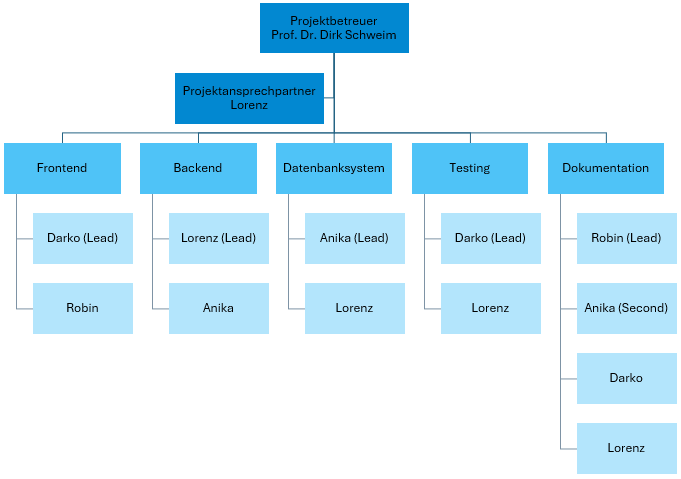
\includegraphics[width=0.8\textwidth]{organigramm}
    \caption{Organigramm}\label{fig:organigramm}
\end{figure}

Das Organigramm weist die Struktur und die Verantwortlichkeiten innerhalb des Projektteams auf.
Es gibt einen klaren Aufbau, der die verschiedenen Rollen und Zuständigkeiten verdeutlicht.

\begin{itemize}
    \item \textbf{Projektbetreuer:}
    \begin{itemize}
        \item \textbf{Prof. Dr. Dirk Schweim:} Der Projektbetreuer steht an oberster Stelle und ist für die Betreuung des Projekts verantwortlich.
    \end{itemize}

    \item \textbf{Projektansprechpartner:}
    \begin{itemize}
        \item \textbf{Lorenz:} Der Projektansprechpartner steht direkt unter dem Projektbetreuer und ist für die Koordination und Kommunikation innerhalb des Teams als auch zum Projektbetreuer zuständig.
    \end{itemize}

    \item \textbf{Frontend:}
    \begin{itemize}
        \item \textbf{Hauptverantwortlich:} Darko
        \item \textbf{Vertretend:} Robin
        \item Die Frontend-Sparte ist für die Gestaltung und Implementierung der Benutzeroberfläche zuständig.
        Darko ist hauptverantwortlich für diese Abteilung, unterstützt von Robin.
    \end{itemize}

    \item \textbf{Backend:}
    \begin{itemize}
        \item \textbf{Hauptverantwortlich:} Lorenz
        \item \textbf{Vertretend:} Anika
        \item Das Backend kümmert sich um die serverseitige Logik und Datenverarbeitung.
        Lorenz ist der Hauptverantwortliche, wobei Anika unterstützend tätig ist.
    \end{itemize}

    \item \textbf{Datenbanksystem:}
    \begin{itemize}
        \item \textbf{Hauptverantwortlich:} Anika
        \item \textbf{Vertretend:} Lorenz
        \item Diese Sparte ist für die Verwaltung und Wartung der Datenbank zuständig.
        Anika hat die Hauptverantwortung, unterstützt von Lorenz.
    \end{itemize}

    \item \textbf{Testing:}
    \begin{itemize}
        \item \textbf{Verantwortlich:} Darko, Lorenz
        \item Testing führt Tests durch, um die Qualität und Funktionalität der Plattform sicherzustellen.
        Darko und Lorenz teilen sich die Verantwortung in diesem Bereich.
    \end{itemize}

    \item \textbf{Dokumentation:}
    \begin{itemize}
        \item \textbf{Hauptverantwortlich:} Robin
        \item \textbf{Vertretend verantwortlich:} Anika
        \item \textbf{Weitere Beteiligte:} Darko, Lorenz
        \item Die Dokumentation wird von allen im Projektteam erstellt und gepflegt.
        Robin ist hauptverantwortlich, Anika übernimmt eine vertretende Rolle, während auch Darko und Lorenz aktiv mitwirken.
    \end{itemize}
\end{itemize}


Diese Struktur weist eine klare Rollenverteilung und entsprechende Vertretung auf, die dem Projektteam ermöglicht, effizient und effektiv an Aufgaben zu arbeiten und ermöglicht eine bessere Zusammenarbeit.



\subsection{Ablaufplanung (Gantt / Netzplan)}\label{subsec:ablaufplan}
Wird in YouTrack erstellt.

Lorenz ipsum dolor sit amet, consetetur sadipscing elitr, sed diam nonumy eirmod tempor invidunt ut labore et dolore magna aliquyam erat, sed diam voluptua.
At vero eos et accusam et justo duo dolores et ea rebum.
Stet clita kasd gubergren, no sea takimata sanctus est Lorem ipsum dolor sit amet.
Lorenz ipsum dolor sit amet, consetetur sadipscing elitr, sed diam nonumy eirmod tempor invidunt ut labore et dolore magna aliquyam erat, sed diam voluptua.
At vero eos et accusam et justo duo dolores et ea rebum.
Stet clita kasd gubergren, no sea takimata sanctus est Lorem ipsum dolor sit amet.
Lorenz ipsum dolor sit amet, consetetur sadipscing elitr, sed diam nonumy eirmod tempor invidunt ut labore et dolore magna aliquyam erat, sed diam voluptua.
At vero eos et accusam et justo duo dolores et ea rebum.
Stet clita kasd gubergren, no sea takimata sanctus est Lorem ipsum dolor sit amet.

\subsection{Stakeholder- und Risikoanalyse}\label{subsec:Stakeholder-Risikoanalyse}
Im Folgenden wurde eine Analyse bezüglich der Stakeholder des Projektes erstellt.
Diese haben unterschiedliche Vorstellungen, Einstellungen und Ansichten zum Projekt.
Ergänzend wurde auch eine Risikoanalyse erstellt, welche zur Übersicht von eventuell eintretenden Problemen verhilft. \par
\newpage %WICHTIG: Nur nötig wenn die Grafik bei der fertigen Doku NICHT unter den oberen Absatz passt! LaTeX schiebt sonst die Grafik weit unpassend im Text runter. @lorack do u know a fix? -Anika

%\Subsubsection{Stakeholderanalyse} \label{Stakeholderanalyse}

\begin{table}[h!]
    \centering
    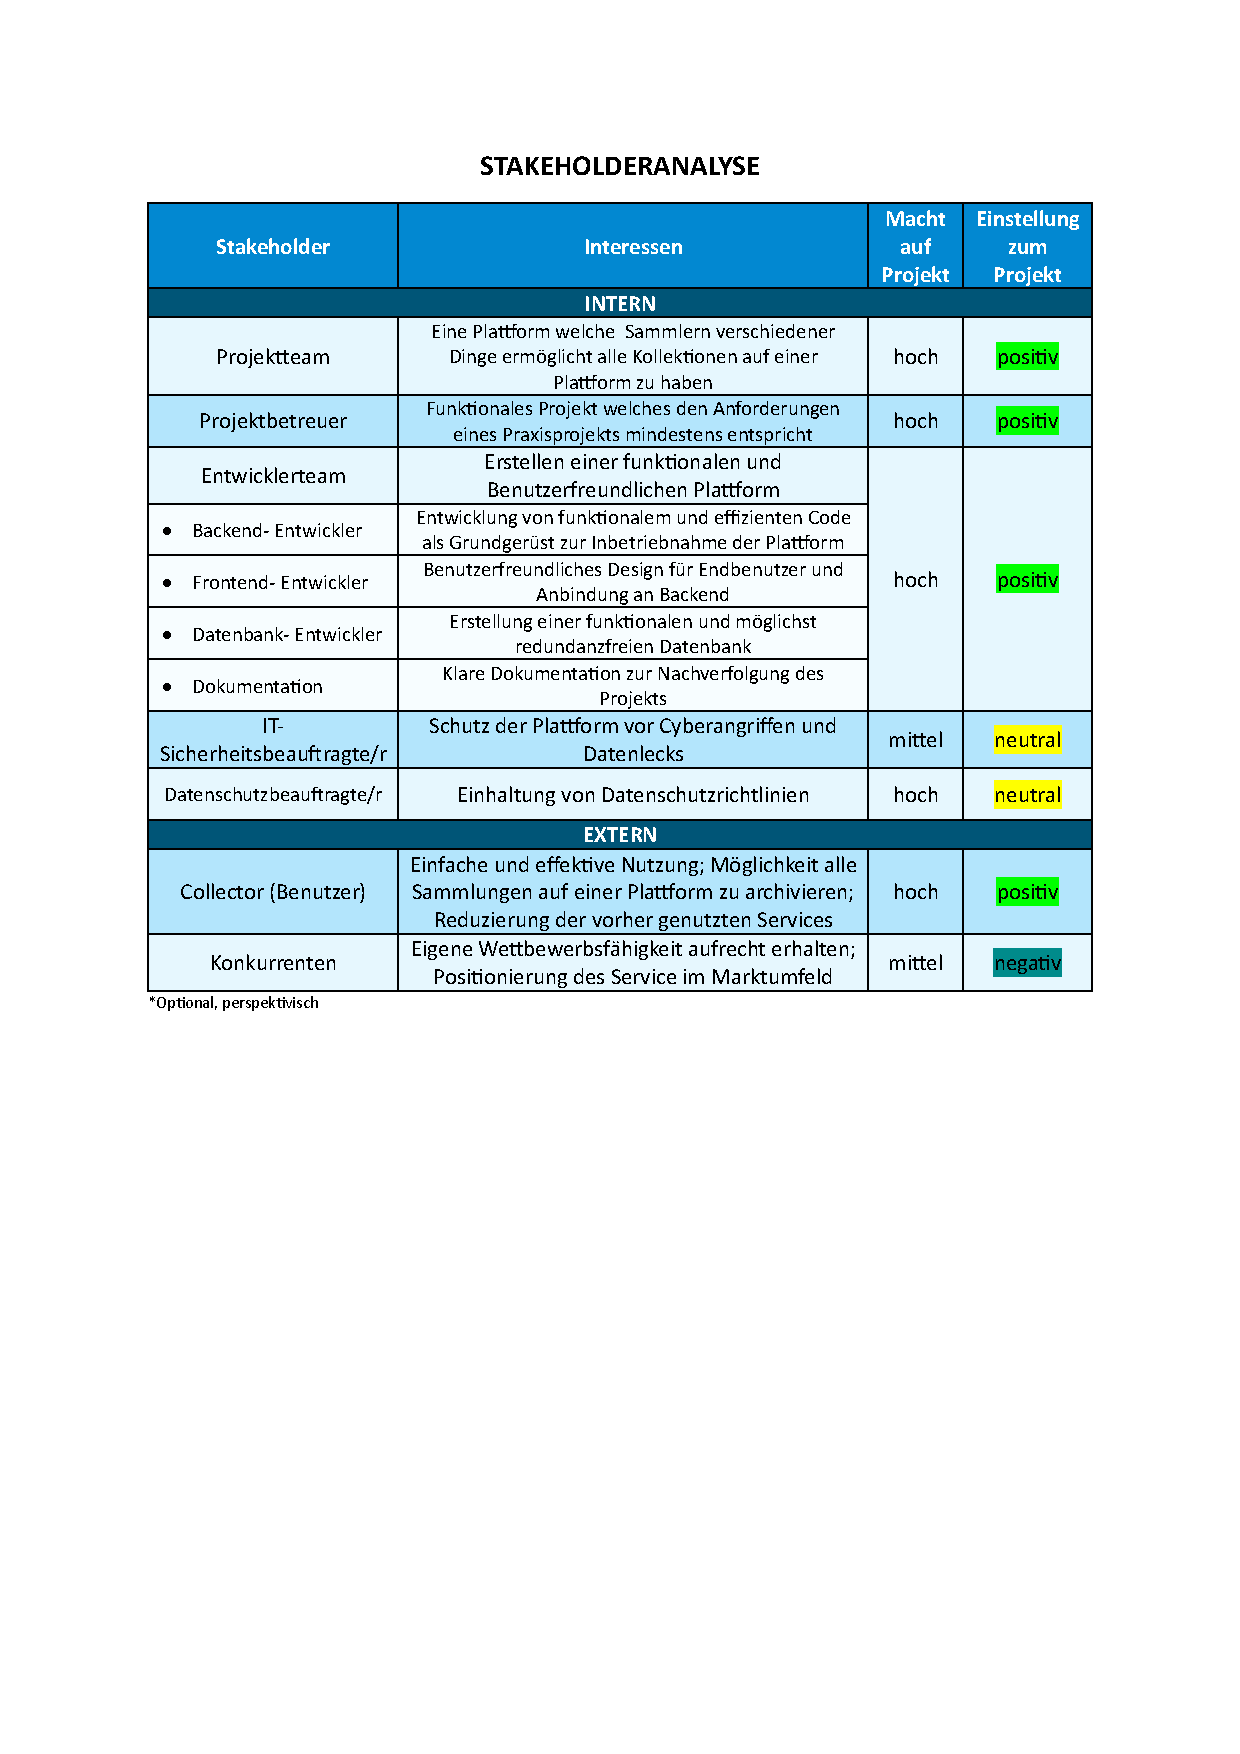
\includegraphics[width=\textwidth, clip, trim=1cm 14.5cm 1cm 3cm]{PM_SH_RISK_ANALYSIS}
    \caption{Stakeholderanalyse}\label{tab:stakegolderanalyse}
\end{table}

Das Projektteam besteht aus Studierenden, die im Rahmen ihres Studiums die Plattform entwickeln.
Das Hauptziel des Teams ist analog zur Zieldefinition von ~\ref{subsec:Zieldefinition}.
Rückblickend auf die Motivation in ~\ref{subsec:Motivation} ist das Team positiv eingestellt. \par

Der Projektbetreuer hat ein starkes Interesse daran, dass das Projekt den Anforderungen eines praxisnahen Studienprojekts entspricht.
Sein Fokus liegt darauf, dass das Projekt nicht nur funktional, sondern auch innovativ und praxisnah ist.
Er hat erheblichen Einfluss auf den Projektverlauf und unterstützt das Team mit wertvollem Feedback und fachlicher Anleitung. \par

Das Entwicklerteam, welches aus dem Projektteam besteht, ist in mehrere spezialisierte Gruppen unterteilt, analog zum Organigramm in ~\ref{subsec:Organigramm}.
Alle Entwicklergruppen haben parallel zum Projektteam-Stakeholder ein hohes Interesse am Projekterfolg und eine positive Einstellung zur Aufgabe, die einzelnen Interessen wurden zwecks persönlicher Lernerfolge nochmal aufgelistet. \par

Als weiterer Stakeholder erweist sich die Rolle der Datenschutzbeauftragten, dessen Hauptaufgabe darin besteht, die Einhaltung der Datenschutzrichtlinien sicherzustellen.
Diese Rolle hat einen hohen Einfluss auf das Projekt, da Datenschutz ein wesentliches, aber auch rechtliches Kriterium für die Plattform darstellt.
Entsprechend ist die Einstellung neutral gehalten. \par


Die Hauptnutzer der Plattform, die Sammler (Collector), stellen einen wesentlichen externen Stakeholder dar.
Ihr Interesse liegt in der einfachen und effektiven Nutzung der Plattform, die es ihnen ermöglicht, ihre Sammlungen zentral zu archivieren und die Nutzung mehrerer vorheriger Dienste zu reduzieren.
Ihre hohe Erwartung und positive Einstellung gegenüber der Plattform sind entscheidend für dessen Akzeptanz und Projekterfolg. \par

%\Subsubsection{Risikoanalyse} \label{Risikoanalyse}
%wichtig: Stake war in Präsens/Futur geschrieben, Risiko bewusst in Vergangenheitsform! >Discuss -Anika

\begin{table}[h!]
    \centering
    \includegraphics[page=2, width=\textwidth, clip, trim=1cm 20cm 1cm 4cm]{PM_SH_RISK_ANALYSIS}
    \caption{Risikoanalyse}\label{tab:risikoanalyse}
\end{table}

Die Entwicklung einer universellen Sammlerplattform wie Collectiqo wies verschiedene Risiken auf, die frühzeitig erkannt und gemindert wurden.
Eine gründliche Risikoanalyse ermöglichte es, potenzielle Herausforderungen zu identifizieren und geeignete Maßnahmen zu entwickeln, um den Projekterfolg sicherzustellen.

\begin{itemize}
    \item \textbf{Technische Herausforderungen:}

    Ein bedeutendes Risiko bei der Entwicklung von Collectiqo lag in der technischen Komplexität des Projekts.
    Da das Projektteam bisher andere Anwendungsfelder bedient hatte, musste das vorhandene Wissen für das Projekt angeglichen und ergänzt werden.
    Um dieses Risiko zu minimieren, war es wichtig, eine gründliche technische Analyse vor Beginn des Projekts durchzuführen.
    Das Projektteam definierte klare und detaillierte Anforderungen und zog so verschiedene technische Lösungen in Betracht, um die Lernkurve entsprechend auf einem möglichen Level, aber dennoch herausfordernd für den eigenen Lernerfolg zu halten.

    \item \textbf{Kommunikationsprobleme:}
    Ein weiteres erhebliches Risiko bestand in möglichen Kommunikationsproblemen innerhalb des Projektteams.
    Da die Teammitglieder verschiedene Arbeitsweisen und Entwicklerstandards ihrer Unternehmen und eigener Erfahrung gewohnt sind, hätte es zu Verständnisproblemen kommen können, welche potentiell zu Verzögerungen, Qualitätsproblemen und einem schlechten Arbeitsklima geführt hätten.
    Um dieses Risiko zu bewältigen, war eine klare und regelmäßige Kommunikation entscheidend.
    Entgegenwirkend hielt das Team regelmäßige Meetings und verwendete YouTrack, um den Fortschritt zu verfolgen und sicherzustellen, dass alle Mitglieder auf dem gleichen Stand sind.

    \item \textbf{Verfügbarkeitsprobleme:}
    Ein weiteres Risiko bestand in möglichen Verfügbarkeitsproblemen, wie dem Ausfall von Services oder Hardware.
    Die Eintrittswahrscheinlichkeit wurde als mittel eingestuft, aber die Auswirkungen könnten den Projektfortschritt erheblich behindern.
    Um dieses Risiko zu minimieren, wurden Fall-Back-Alternativen und Lokalkopien erstellt, um die Arbeit auch bei Ausfällen fortsetzen zu können.
\end{itemize}



\subsection{Kosten- und Aufwandsplanung}\label{subsec:Kosten-Aufwandsplanung}
Lorenz ipsum dolor sit amet, consetetur sadipscing elitr, sed diam nonumy eirmod tempor invidunt ut labore et dolore magna aliquyam erat, sed diam voluptua.
At vero eos et accusam et justo duo dolores et ea rebum.
Stet clita kasd gubergren, no sea takimata sanctus est Lorem ipsum dolor sit amet.
Lorenz ipsum dolor sit amet, consetetur sadipscing elitr, sed diam nonumy eirmod tempor invidunt ut labore et dolore magna aliquyam erat, sed diam voluptua.
At vero eos et accusam et justo duo dolores et ea rebum.
Stet clita kasd gubergren, no sea takimata sanctus est Lorem ipsum dolor sit amet.
Lorenz ipsum dolor sit amet, consetetur sadipscing elitr, sed diam nonumy eirmod tempor invidunt ut labore et dolore magna aliquyam erat, sed diam voluptua.
At vero eos et accusam et justo duo dolores et ea rebum.
Stet clita kasd gubergren, no sea takimata sanctus est Lorem ipsum dolor sit amet.

\subsection{Tools}\label{subsec:Tools}
Lorenz ipsum dolor sit amet, consetetur sadipscing elitr, sed diam nonumy eirmod tempor invidunt ut labore et dolore magna aliquyam erat, sed diam voluptua.
At vero eos et accusam et justo duo dolores et ea rebum.
Stet clita kasd gubergren, no sea takimata sanctus est Lorem ipsum dolor sit amet.
Lorenz ipsum dolor sit amet, consetetur sadipscing elitr, sed diam nonumy eirmod tempor invidunt ut labore et dolore magna aliquyam erat, sed diam voluptua.
At vero eos et accusam et justo duo dolores et ea rebum.
Stet clita kasd gubergren, no sea takimata sanctus est Lorem ipsum dolor sit amet.
Lorenz ipsum dolor sit amet, consetetur sadipscing elitr, sed diam nonumy eirmod tempor invidunt ut labore et dolore magna aliquyam erat, sed diam voluptua.
At vero eos et accusam et justo duo dolores et ea rebum.
Stet clita kasd gubergren, no sea takimata sanctus est Lorem ipsum dolor sit amet.

\begin{itemize}
    \item one
    \item two
    \item three
\end{itemize}

    \newpage

    \section{Entwurf und Design}\label{sec:entwurf-und-design}

Dieses Kapitel beschreibt die Entwürfe in Abschnitt~\ref{subsec:entwurf}.
Darauf hin wird auf die Zielplattform in Abschnitt~\ref{subsec:zielplattform} eingegangen.

\subsection{Entwurf}\label{subsec:entwurf}

In der Entwurfsphase wurden die wesentlichen Strukturen der Lösung entworfen, um einen Überblick für die Entwicklungsphase zu erstellen.
Ein Mockup des Webfrontends wurde erstellt, wovon Ausschnitte in Abbildungen~\ref{fig:mockup1},~\ref{fig:mockup2} und~\ref{fig:mockup3} zu sehen sind.

\begin{figure}[h]
    \centering
    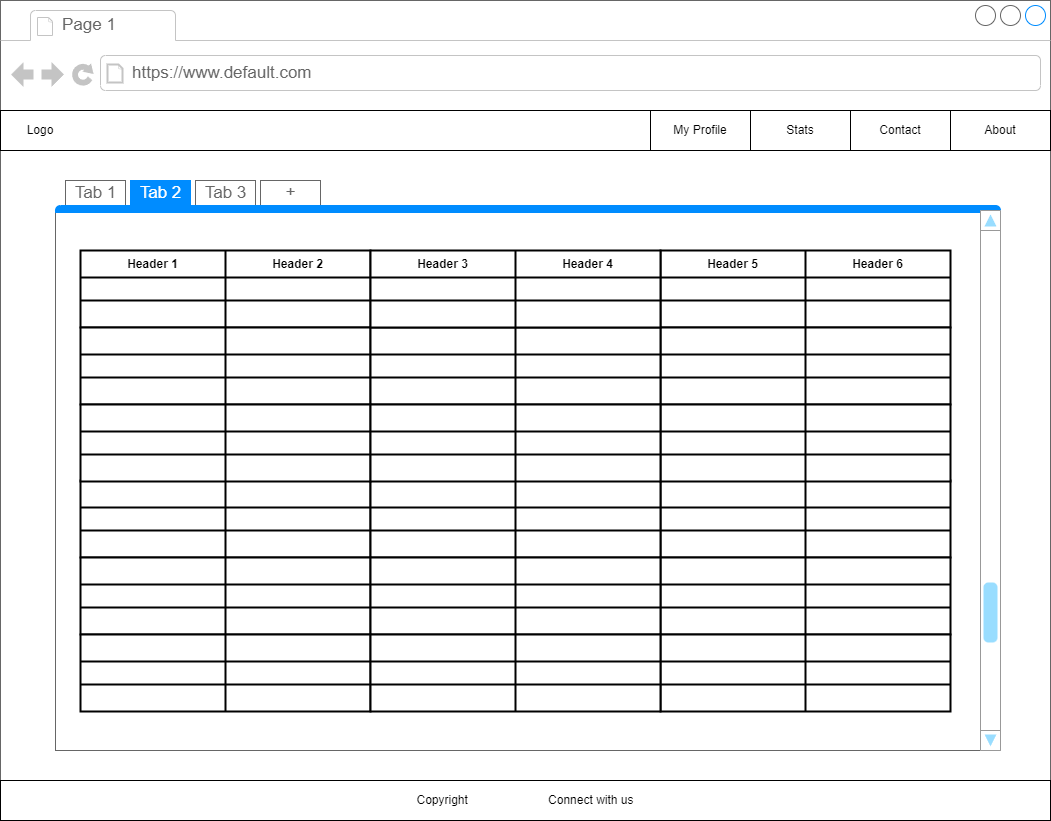
\includegraphics[width=0.55\textwidth]{loggedIn_starting_site}
    \caption{Mockup der Startseite nach Login}
    \label{fig:mockup1}
\end{figure}

\begin{figure}[h]
    \centering
    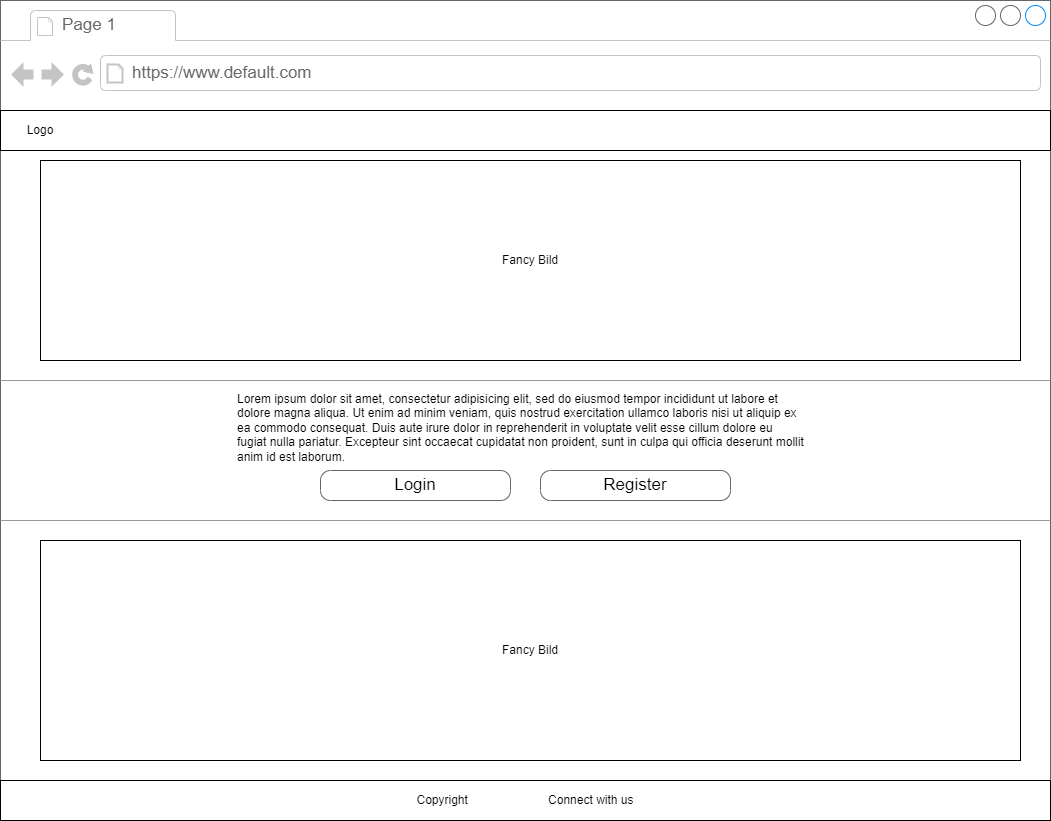
\includegraphics[width=0.55\textwidth]{Starting_site}
    \caption{Mockup der allgeminen Startseite}
    \label{fig:mockup2}
\end{figure}

\begin{figure}[h]
    \centering
    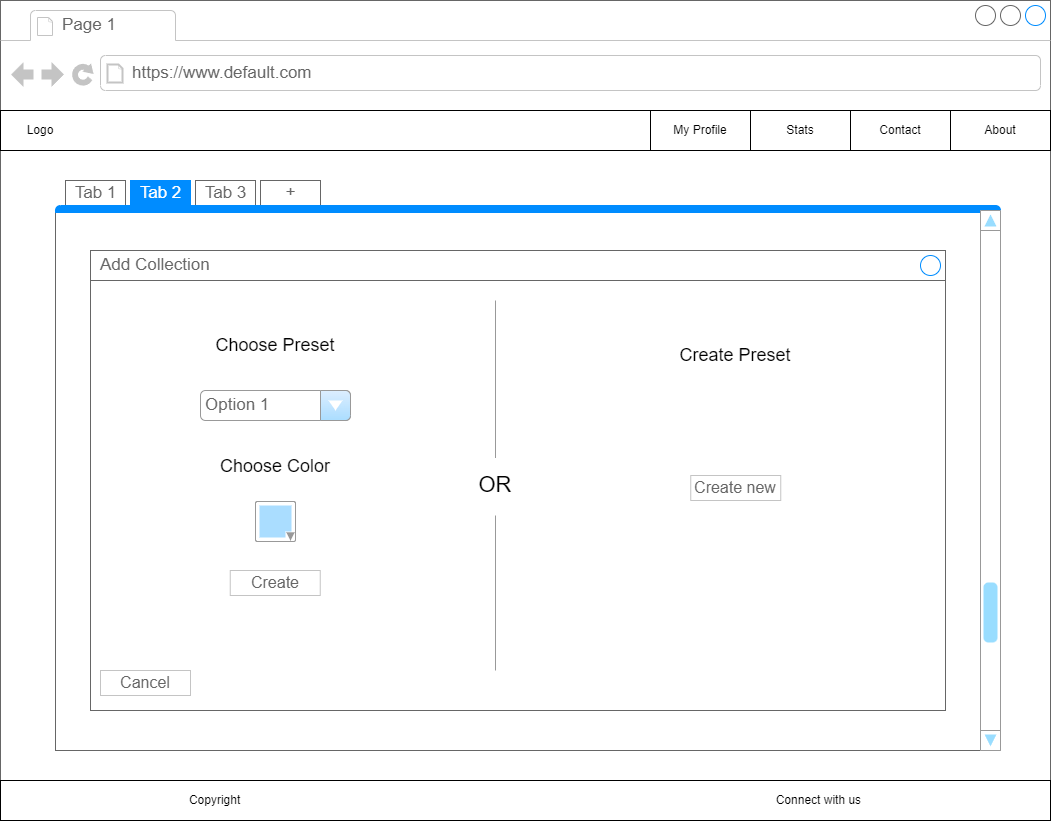
\includegraphics[width=0.55\textwidth]{add_collection_pop_up}
    \caption{Mockup des Popups zur Erstellung einer Sammlung}
    \label{fig:mockup3}
\end{figure}

\subsection{Zielplattform}\label{subsec:zielplattform}

Die Lösung ist eine Webanwendung, welche zukunftsorientiert online im Web verfügbar sein könnte.
Als Programmiersprache für die Webanwendung wurde JavaScript verwendet.
JavaScript bot sich an, da diese Sprache weitverbreitet und plattformunabhängig für die Webentwicklung ist.
JavaScript ermöglichte eine Integration des Webfrontends in verschiedenen Browsern und erleichterte die Implementierung von interaktiven Funktionen.
Zudem bot es die Möglichkeit, verschiedene Bibliotheken und Frameworks zu nutzen, um die Lösung effizient und ressourcenschonend zu gestalten.
Im Entwurfsprozess entschieden wir uns für die Verwendung von Node.js, da Node.js Frameworks und Bibliotheken vielseitige Funktionalitäten abdecken und nützlich sind, um die Daten aus der Datenbank zu verarbeiten, Routen zu definieren und HTTP-Requests auszuführen.

\begin{itemize}[itemsep=1em, leftmargin=*]
    \item \textbf{Client-Seite:} Die Client-Seite unserer Anwendung nutzt HTML, CSS und JavaScript, um eine interaktive und benutzerfreundliche Oberfläche bereitzustellen.
    \item \textbf{Abhängigkeiten Client-Seite:}
    \begin{itemize}[itemsep=1em, leftmargin=*]
        \vspace{1em}
        \item \textbf{node:} Als Laufzeitumgebung sorgt Node.js dafür, dass JavaScript-Code außerhalb des Browsers ausgeführt werden kann, was besonders für die Entwicklung und das Testen der Anwendung nützlich ist.
        \item \textbf{axios:} Diese Bibliothek wird für HTTP-Anfragen verwendet, um Daten zwischen Client und Server auszutauschen.
        \item \textbf{ejs:} Embedded JavaScript (EJS) dient als Template-Engine, die HTML mit dynamischen Inhalten aus JavaScript-Datenquellen rendert.
        \item \textbf{ejs-lint:} Ein Tool zur Überprüfung und Validierung von EJS-Templates, um Fehler frühzeitig zu erkennen und zu beheben.
    \end{itemize}
    \item \textbf{Funktionalitäten:} Die Client-Seite umfasst die Benutzeroberfläche (UI) und enthält Eingabeformulare zur Erfassung und Bearbeitung der Sammlung.
    Sie ermöglicht eine dynamische Aktualisierung der Inhalte basierend auf Benutzerinteraktionen, was eine reaktive und intuitive Nutzung der Anwendung gewährleistet.
    \item \textbf{Server-Seite:} Die Server-Seite unserer Anwendung verwendet Node.js und Express.js, um eine robuste und skalierbare Backend-Umgebung zu schaffen.
    \item \textbf{Abhängigkeiten Server-Seite:}
    \begin{itemize}[itemsep=1em, leftmargin=*]
        \vspace{1em}
        \item \textbf{node:} Als Laufzeitumgebung sorgt Node.js für die Ausführung von JavaScript auf dem Server.
        \item \textbf{express:} Dieses Web-Framework wird verwendet, um Webanwendungen und APIs zu erstellen, die HTTP-Anfragen und -Antworten verarbeiten.
        \item \textbf{express-session:} Diese Middleware verwaltet Benutzersitzungen und stellt sicher, dass die Sitzungsdaten sicher und effizient gespeichert werden.
        \item \textbf{jsonwebtoken:} Diese Bibliothek implementiert JSON Web Tokens (JWT) für die Authentifizierung und Autorisierung von Benutzern.
        \item \textbf{dotenv:} Diese Bibliothek hilft bei der Verwaltung von Umgebungsvariablen, was die Konfiguration der Anwendung vereinfacht und sicherer macht.
        \item \textbf{mysql2:} Diese Bibliothek ermöglicht die Anbindung an eine MySQL-Datenbank.
        \item \textbf{mongodb:} Diese Bibliothek ermöglicht die Anbindung an eine MongoDB-Datenbank.
        \item \textbf{bcryptjs:} Diese Bibliothek wird verwendet, um Passwörter zu hashen und somit die Sicherheit der Benutzerdaten zu erhöhen.
    \end{itemize}
    \item \textbf{Routen:} Auf der Client-Seite sind definierte Endpunkte für CRUD-Operationen (Create, Read, Update, Delete) auf den gesammelten Objekten implementiert.
    Diese Routen sorgen für eine strukturierte und nachvollziehbare Datenverwaltung und -darstellung.
    Auf der Server-Seite sind ebenfalls definierte Endpunkte für CRUD-Operationen auf den gesammelten Objekten implementiert.
    Diese Endpunkte ermöglichen die Datenverwaltung und -verarbeitung und stellen sicher, dass die Anwendung auf Anfragen der Client-Seite effizient reagiert.
    \item \textbf{Docker und Containerisierung:} Für die Konfiguration der Container werden Dockerfiles verwendet, die die Umgebung und Abhängigkeiten jeder Komponente definieren.
    Docker-Compose wird zur Orchestrierung mehrerer Container eingesetzt, um eine konsistente und leicht zu verwaltende Infrastruktur zu gewährleisten.
    Die Nutzung von Docker sorgt für konsistente Umgebungen zwischen Entwicklung und Produktion, was die Fehleranfälligkeit reduziert.
    Darüber hinaus ermöglicht Docker eine einfache Verteilung und Skalierbarkeit der Anwendung, da Container schnell gestartet, gestoppt und vervielfältigt werden können.
    \item \textbf{Kommunikation zwischen Client und Server:} Die Anwendung nutzt eine RESTful API, um klar strukturierte API-Endpunkte zu definieren, die über HTTP-Methoden (GET, POST, PUT, DELETE) zugänglich sind.
    Diese Endpunkte ermöglichen eine standardisierte und effiziente Kommunikation zwischen Client und Server.
    JSON wird als Datenformat für den Datenaustausch zwischen Client und Server verwendet.
    JSON ist leichtgewichtig und einfach zu parsen, was die Effizienz und Leistung der Anwendung erhöht.
    \item \textbf{Gesamtbetrachtung:} Die Kombination aus Client-Server-Architektur, Node.js/Express für die Backend-Logik, und der Containerisierung mit Docker ermöglicht eine skalierbare, flexible und leicht wartbare Anwendung.
    Diese Architektur unterstützt eine klare Trennung der Verantwortlichkeiten zwischen Client und Server und sorgt für eine konsistente und isolierte Umgebung für die verschiedenen Komponenten der Anwendung.
    Die detaillierte Auflistung der Abhängigkeiten gewährleistet Transparenz und erleichtert die Wartung sowie Weiterentwicklung der Anwendung.
\end{itemize}

    \newpage

    \section{Durchführung / Implementierung}\label{sec:durchfuehrung-implementierung}

Die Entwicklung des Projekts lässt sich grob ich zwei Phasen aufteilen.
Die erste Phase ist die Planungsphase, in welcher die Anforderungen an das Projekt definiert und die Architektur der Anwendung festgelegt wurde.
Die Resultate aus dieser Phase wurden in den vorherigen Kapiteln beschrieben.
Beendet wurde diese Phase mit der ersten Präsentation des Projekts, in welcher die Projektidee vorgestellt wurde.
Die zweite Phase ist die Durchführungsphase, in welcher die Anwendung umgesetzt wurde und welche im diesem Kapitel beschrieben wird.
Gestartet hat diese Phase direkt nach dem Ende der ersten Phase, nach welcher die Erlaubnis zur Durchführung des Projekts erteilt wurde.
Hierbei wurden die Aufgaben basierend auf dem Organigramm verteilt.
Während die Verantwortlichen für die Datenbank und das Backend sich des Öfteren Abstimmen mussten, konnte das Frontend-Team weitestgehend unabhängig arbeiten.
Jedes Teammitglied hat sich selbstständig in die Thematiken eingearbeitet, die für die Umsetzung ihres Verantwortungsbereichs nötig waren.

Der übliche Ablauf während der Durchführungsphase war es, dass sich das Team einmal in der Woche zusammengesetzt hat um den aktuellen Stand der Projektbausteine zu besprechen.
Hierbei wurde abgesprochen, welche Aufgaben bis zum nächsten Treffen erledigt werden sollten.
Mussten Abschnitte aus einzelnen Bereichen zusammengeführt werden, wurde dies in einem separaten Meeting besprochen, woran nur die verantwortlichen Teammitglieder teilgenommen haben.
Die Aufgaben wurden mit YouTrack verwaltet, wodurch immer ein klares Verständnis über die Aufgabenverteilung herrschte.
Das Dashboard wurde während den Team Meetings basierend auf dem Stand und der Verteilung aktualisiert.
Die Aufgaben wurden in Open, In Progress, To Be Reviewed und Done unterteilt.
Ein Einblick in die YouTrack Aufgabenverwaltung ist in Abbildung~\ref{fig:youtrack_screenshot_agile_board} zu sehen.

\begin{figure}[h]
    \centering
    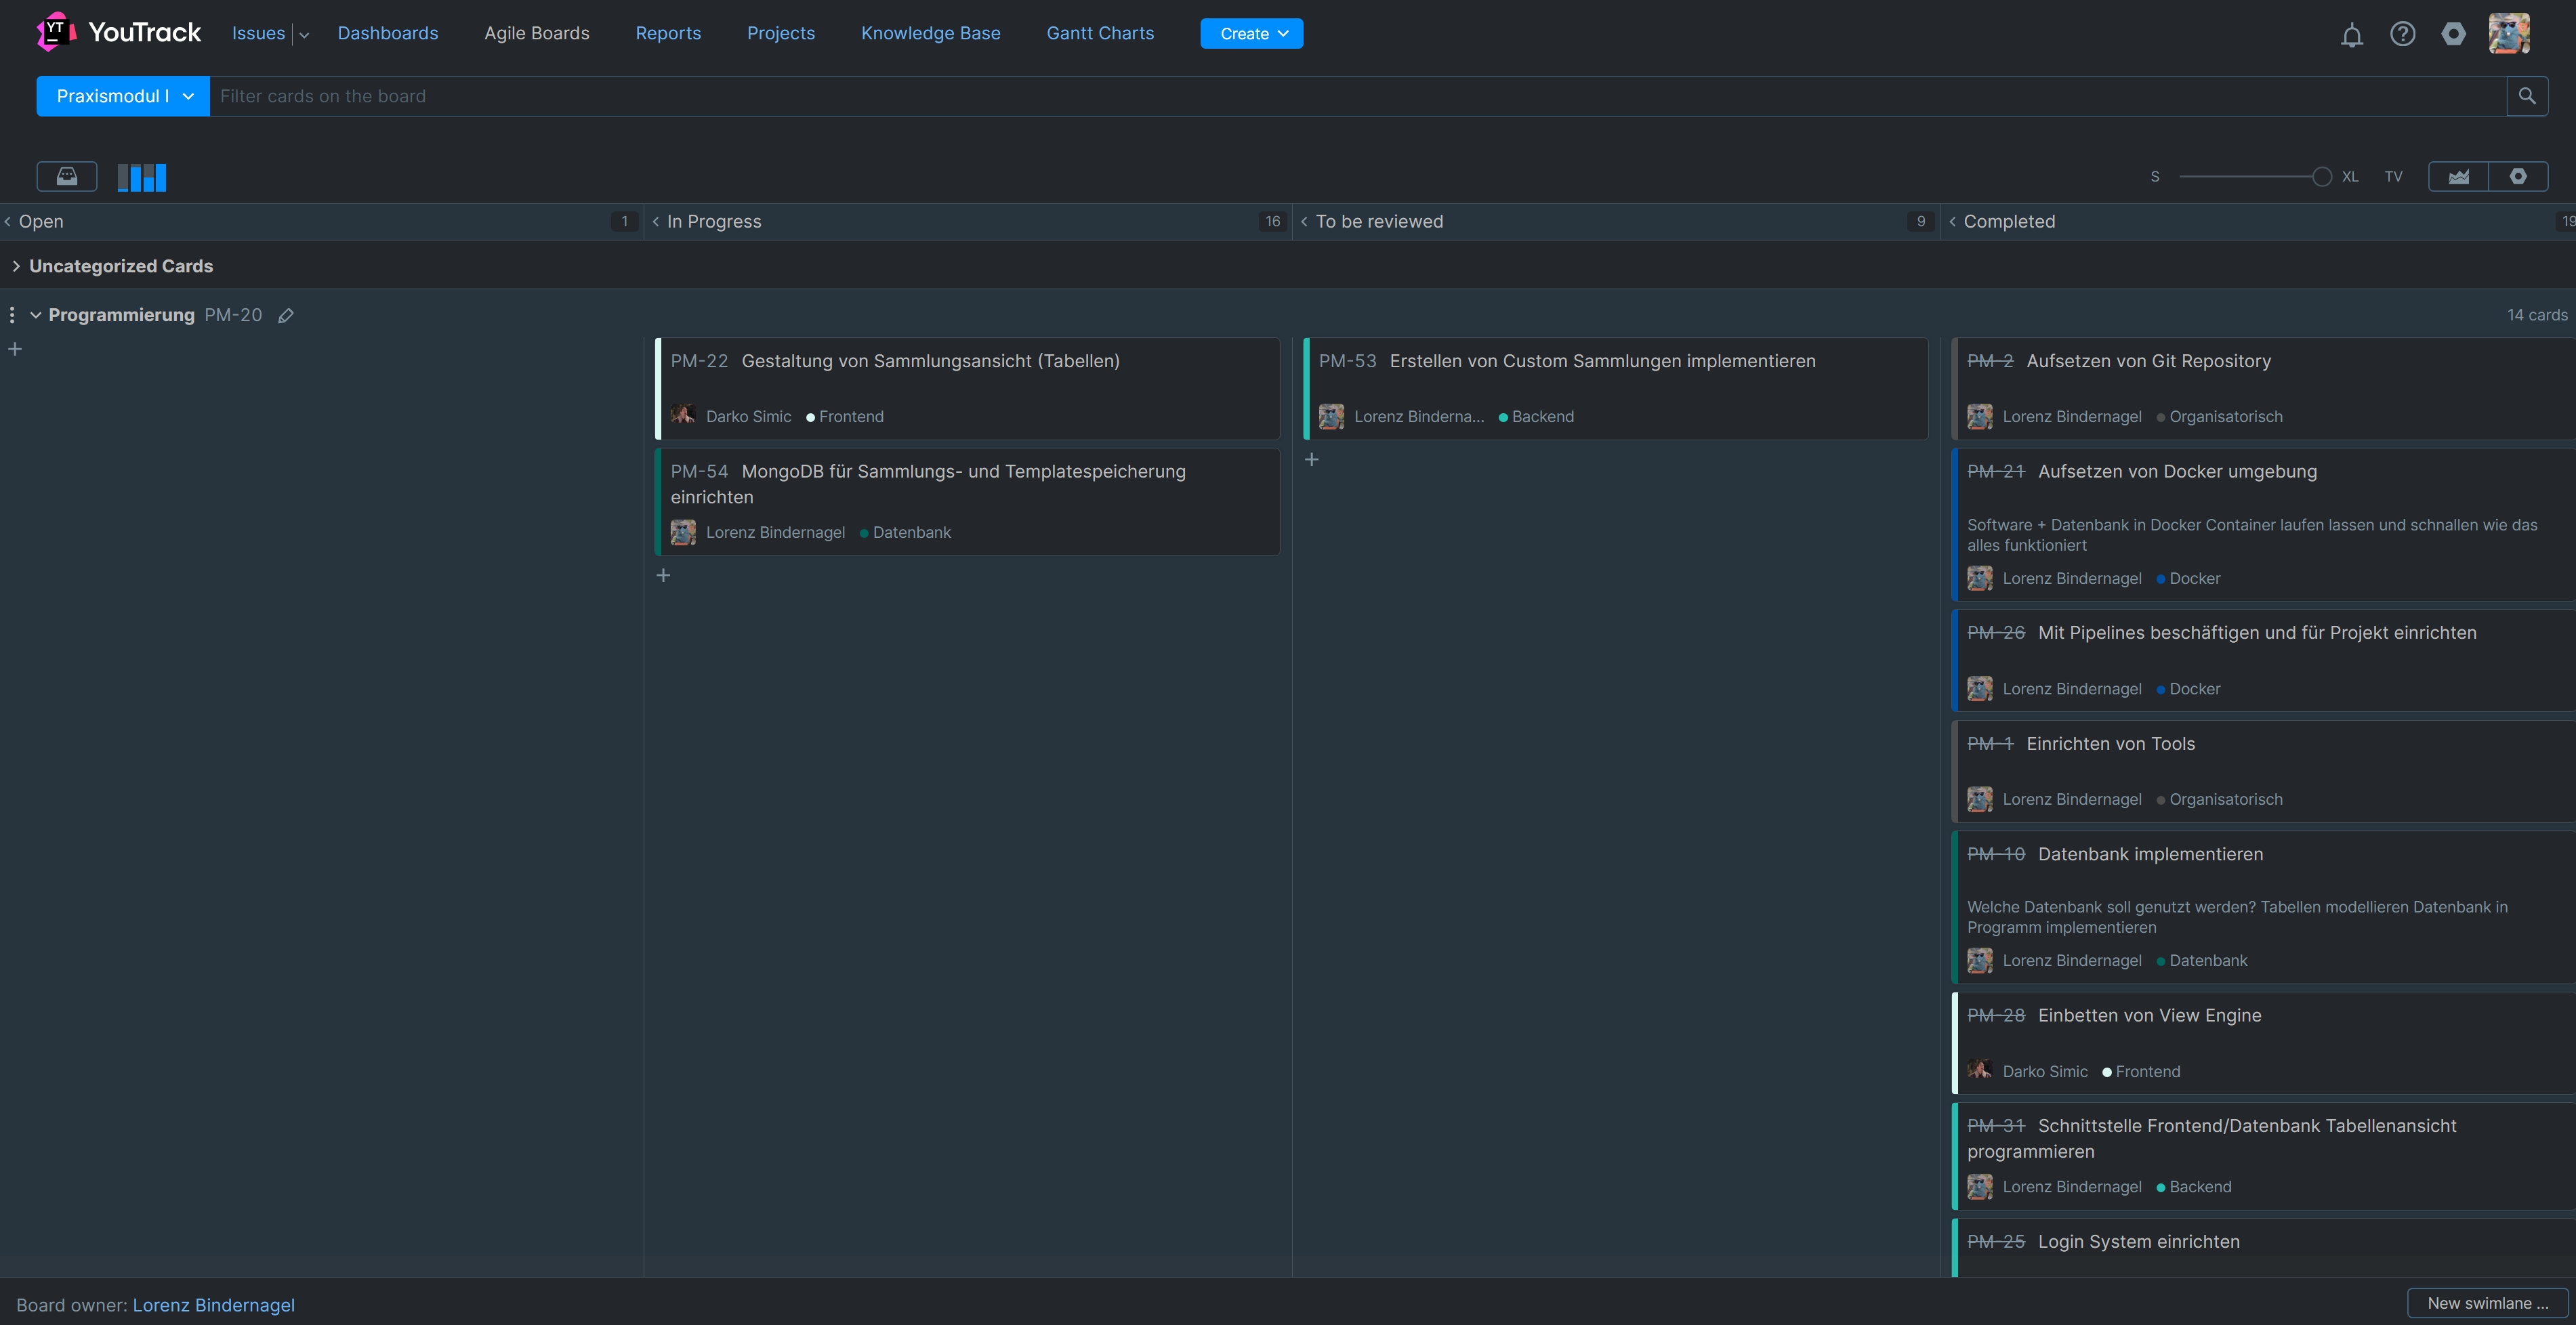
\includegraphics[width=1\textwidth]{youtrack_screenshot_agile_board}
    \caption{Screenshot des Agile Dashboards in YouTrack}
    \label{fig:youtrack_screenshot_agile_board}
\end{figure}

\subsection{Entwicklung des Webfrontends}\label{subsec:entwicklung-des-webfrontends}
Die Entwicklung des Webfrontends konzentrierte sich auf die Erstellung einer benutzerfreundlichen Oberfläche und alle nötigen Grundfunktionen und Strukturen.
Mithilfe von HTML, CSS und EJS wurde eine schlichte Webseite gestaltet.

Das Herzstück der Webseite ist das Anlegen eigener Collections, welche dynamisch mit Daten aus der hinterlegten MongoDB Datenbank befüllt wird.
Die Datenbank wird dabei durch JavaScript und dessen Frameworks und Bibliotheken angesprochen, welche wiederum durch das Frontend angestoßen werden.
Für das Webfrontend wurde eine Express-Anwendung in Node.js erstellt, welche auf statische Dateien (CSS, JS, Bilder) aus dem Ordnerverzeichnis zugreift.
Die Verwendung von Node.js ermöglicht das Definieren von HTTP Routen mit JavaScript, um so durch die verschiedenen Seiten der Webseite navigieren zu können und serverseitige Funktionen aufzurufen.

EJS wurde als Template-Engine verwendet, um die Integration von JavaScript innerhalb von HTMLDokumenten zu ermöglichen und somit auch seine Sammlungen abrufen zu können.
Dies erlaubte eine flexible und dynamische Gestaltung der Webseite, insbesondere durch die Verwendung von EJS-Tags wie \grqq\textless{}\%=\%\textgreater{}\grqq{}, die es ermöglichte, serverseitige Variablen oder Ausdrücke direkt in die HTML-Struktur einzufügen.
In diesem Fall wurden die Collections aus der Datenbank abgerufen und über eine Schleife in der EJS-Vorlage gerendert und werden einmal in einer Übersicht angezeigt.
In dieser Übersicht hat man die Möglichkeit eine beliebig angelegte Collection anzuklicken um so diese anzuschauen oder auch zu bearbeiten.

\subsection{Entwicklung des Backends}\label{subsec:EntwicklungDesBackends}
Der erste Schritt bei der Backend entwicklung war es, einen geeigneten Startpunkt zu finden.
Hierbei wurde entschieden, dass zuerst eine Implementierung der Datenbankverbindung erfolgen sollte, da diese als Grundlage für die weitere Entwicklung dient.
Dies wurde mit der Bibliothek mysql2 realisiert, welche eine erweiterte Funktionalität gegenüber der Standardbibliothek bietet und diverse Probleme behebt.
Diese implementierung war erst möglich, nachdem die Grundstruktur der Datenbank aufgesetzt wurde.
Einen Einblick in den Code gibt Listing\ref{lst:connecttomysql}.

\lstinputlisting[language=JavaScript,label={lst:connecttomysql}]{../server/dbConnections/connectToMYSQL.js}

Als Nächstes wurde sich dazu entschieden, ein einfaches Sign Up und Login System zu programmieren.
Hierbei wurde auf die Bibliothek bcrypt zurückgegriffen, welche das Hashen von Passwörtern erleichtert.
Die SQL queries, die hier genutzt werden, wurden ebenfalls mit der mysql2 Bibliothek realisiert.
Die einzigen Nutzerdaten, die hierbei gespeichert werden, sind der Username, die E-Mail und das Passwort.
Beim Login wurde darauf geachtet, das Nutzer Username und E-Mail benutzen können, um sich einzuloggen.
Ein Einblick in den Code gibt Listing\ref{lst:login}.

\lstinputlisting[languange=JavaScript,label={lst:login}]{../server/authentication/loginHandler.js}

Nun stellte sich die Frage, wie es möglich ist, dass Nutzer nur auf ihre eigenen Sammlungen zugreifen können.
Beim Recherchieren sind wir auf das Konzept von Sessions gestoßen und wollten diese ausprobieren.
Die erste Anwendung fanden Sessions im Speichern des Usernamens in einer Session Variable, nachdem der User sich angemeldet hat.
Der nächste Schritt war es, die Sammlungen eines Nutzers basierend auf dem Usernamen aus der Datenbank zu laden.
Zuvor muss jedoch erstmal eine Funktion implementiert werden, mit der Sammlungen angelegt werden können.
Hierzu muss zuerst die Datenbank implementiert werden, in welcher die Sammlungen gespeichert werden.
Als Datenbank für die Sammlungen wurde sich für MongoDB entschieden, welches im Kapitel~\ref{subsec:entwicklung-der-datenbank-und-datenstruktur} genauer erläutert wird.

Nur das Anlegen von Sammlungen reicht natürlich nicht, weshalb weitere Funktionen im Backend implementiert wurden, die diverse grundlegende Funktionen ermöglichen.
Hierzu zählen das Löschen von Sammlungen, das Hinzufügen von Items zu Sammlungen und das Löschen von Items aus Sammlungen.
Außerdem wurde eine separate Funktion implementiert, die das Erstellen einer Sammlung direkt von einem Template aus ermöglicht.


Während der Entwicklung des Backends kam es jedoch auch des Öfteren zu Herausforderungen.
Eine dieser Stellen war der Umgang mit Docker Containern.
Ein gewisses Grundverständnis war vorhanden, doch praktische Erfahrung war im gesamten Team nicht vorhanden.
Zwar was das Hochfahren einer Datenbank in einem Container schnell erreicht, doch ein Verständnis für Datenpersistenz und Volumes zu entwickeln, benötigte seine Zeit.
Auch im späteren Verlauf des Projekts, als es darum ging alle Applikationskomponenten in einer Docker-Compose Datei zusammenzuführen, stellte sich als Herausforderung heraus.
Wie sich Dockerfiles in dem ganzen System einordnen und wo sie genutzt werden, war ebenfalls neu für das Team.
Allgemein hat das Einfinden in Docker dem Team mehr Zeit als erwartet abverlangt.

Eine weitere Herausforderung war das Einfinden in die verschiedenen Bibliotheken, die bei Webentwicklung mit JavaScript genutzt werden.
Zwar wurde in der Planung bereits einige Bibliotheken festgelegt, die genutzt werden sollten, doch während der Entwicklung kamen einige neue hinzu.
Ein Beispiel hierfür ist die Bibliothek express-session, die für das Session-Management genutzt wird.
Da zur Planung noch kein detailliertes Verständnis darüber vorhanden war, welche Komponenten bei der Entwicklung einer solchen Anwendung benötigt werden, wurden Thematiken wie Session Management erst während der Entwicklung entdeckt.
Hierdurch kam es an einigen Stellen zu steilen, jedoch unvermeidbaren Lernkurven, die jedoch auch entsprechenden zeitlichen Aufwand mit sich gebracht haben.

Da das Team zuvor noch nie eine Webanwendung entwickelt hat, fehlte es an Verständnis, wie viel Komponenten Teil einer solchen Anwendung sind.
So kam es, dass während der Entwicklung immer wieder neue Komponenten entdeckt wurden, die in der Planung nicht berücksichtigt wurden.
Ein konkretes Beispiel hierfür ist das Session-Management.

\subsection{Entwicklung der Datenbank und Datenstruktur}\label{subsec:entwicklung-der-datenbank-und-datenstruktur}

Bei der Einrichtung der Datenbank stellt sich als erste Hürde der Umgang mit Docker Container heraus.
Zwar waren grundlegende Kentnisse über Docker vorhanden, doch eine Datenbank praktisch in einem Container hochzufahren und diese dann mit dem Code und der Programmierumgebung zu verknüpfen, war eine neue Herausforderung.
Hierzu mehr in Kapitel~\ref{sec:Herausforderungen}.
Wie in der Planung entschieden, sollen zwei Datenbanken genutzt werden - eine MySQL Datenbank für strukturierte Daten und eine MongoDB Datenbank für unstrukturierte Daten.
Im ersten Schritt wurde die MySQL Datenbank aufgesetzt und mit Tabellen für Nutzerdaten und den drei Pre-Sets für Sammlungen befüllt.
Die Nutzerdaten beinhalten Username, E-Mail und Passwort.
Für die Themenbereiche Video Spiele und Parfum wurden jeweils eine Tabelle erstellt, die für das Thema passende Spalten beinhalten.

Als Datenbank für die Sammlungen wurde sich für eine MongoDB Datenbank entschieden.
Dies liegt daran, dass MongoDB eine dokumentenorientierte Datenbank ist, die sich gut für die Speicherung von unstrukturierten Daten eignet.
Die Daten der Sammlungen sind unstrukturiert, da sie sich je nach Thema unterscheiden.
Dies ist das erste Mal, dass das Team mit einer dokumentenorientierten Datenbank arbeitet, daher musste erstmal ein Verständnis über den Aufbau einer solchen Datenbank geschaffen werden.
Zunächst wurde versucht vergleiche mit einer SQL Datenbank herzustellen, wobei schnell auffiel, dass Konzepte wie Schemata hier Collections sind.
Das Integrieren der Datenbank in der Programmierumgebung war schnell erledigt, da dies analog zu der MySQL Datenbankverbindung erfolgt ist.
Das Auslesen und schreiben von Daten in die Datenbank war dank der MongoDB Bibliothek einfach erledigt.
Funktionen für die Verbindung mit der Datenbank wurden in einer separaten Datei ausgelagert.

Die Herausforderungen, die beim Einrichten des Datenbanksystems entstanden sind, teilen sich in zwei Punkte auf.
Der erste Punkt hängt damit zusammen, dass das Einrichten der Datenbanken gleichzeitig die erste praktische Nutzung von Docker Containern war.
Somit musste erstmal ein Verständnis dafür entwickelt werden, wie vom Hostsystem auf die Container zugegriffen werden kann und wie Daten persistiert werden.
Da die Datenbanken vorgefertigten Inhalt benötigten, wie bspw.\ die Templates für die Sammlungen in der MongoDB oder das Datenbankschema für User in der MySQL Datenbank, musste sich angeeignet werden, wie Docker Images erstellt werden können.
Darüber hinaus musste recherchiert werden, wie man solche Images hosten kann, sodass jeder beim Starten der Docker Compose Datei die Datenbanken mit den nötigen Inhalten erhält.

\subsection{Verbinden des Frontends und Backends}\label{subsec:verbinden-des-frontends-und-backends}

\subsection{Implementieren von Tests}\label{subsec:implementieren-von-tests}

Um Teile des Backends zu testen, bevor diese mit dem Frontend verbunden werden konnten, wurde versucht Unit-Tests zu schreiben.
Dieser Prozess stellte sich als komplizierter heraus als gedacht, da das Team zuvor noch nie mit Tests für JavaScript gearbeitet hat.
So konnten zwar einfache Unit-Tests für das Login System geschrieben werden, jedoch Integrationstests, in welchen die Datenbank angesprochen wird, stellten sich als schwierig heraus.
Ein exemplarischer Test für das Login System ist in Listing~\ref{lst:loginTest} zu sehen.


\lstinputlisting[language=JavaScript, firstline=15, lastline=32, label={lst:loginTest}]{../test/loginHandler.test.js}


Auch gab es Probleme damit, eine Datei für Umgebungsvariablen für Testdatenbanken korrekt in die Tests mit einzubinden.
Erst nach längerer Recherche stellte sich heraus, dass Umgebungsvariablen für jest Tests in einer separaten Config Datei definiert werden müssen und nicht wie die normale .env Datei in den Code eingebunden werden konnte.
Auch mit den Mock Funktionen von jest musste sich erst eingearbeitet werden.
An dieser Stelle wurde sich dazu entschieden, die implementierung von Tests für alle Backend Funktionen abzubrechen, da der Aufwand zu groß war und die Zeit zu knapp.
Der zeitliche Aufwand für das Einrichten der automatisierten Tests war zu hoch, vor allem im Vergleich zu dem zeitlichen Aufwand den ein manueller Test benötigt hätte.
Manuelle Tests wurden durchgeführt, als das Backend mit dem Frontend verbunden war.
Ein Nachteil, der dadurch entstanden ist, ist dass Funktionen öfters nachträglich angepasst werden mussten, was die Verbindung zum Frontend zeitaufwendiger machte.
    \newpage

    \section{Rückblick / Retrospektive}\label{sec:rueckblick-retrospektive}

Dieser Abschnitt gibt einen Vergleich zwischen den geplanten Zielen und den tatsächlich erreichten Zielen.
Daraufhin wird geschaut, welche Verbesserungen in der Durchführung nächstes Semester umgesetzt werden könnten, sowie welche neuen Kenntnisse .
Schlussendlich wird ein Ausblick auf zukünftige Ziele und Funktionen gegeben, wovon einige aus den geplanten Zielen für dieses Semester übernommen werden und einige neue hinzukommen, die dem Team bei der Umsetzung eingefallen sind.

\subsection{Abweichungen der geplanten Ziele}\label{subsec:abweichungen-der-geplanten-ziele}
Während der Umsetzung wurden immer wieder die Definitions of done in Betracht gezogen.
Dieses Kapitel betrachtet die einzelnen Ziele und schaut, ob diese erreicht wurden und was der aktuelle Stand in der Umsetzung ist.
Hierbei wurden die Ziele auf die beschränkt, die direkt etwas mit der Umsetzung des Projekts zu tun haben.
Ziele wie die erfolgreiche Abgabe des Projekts wurden somit außen vor gelassen.

\begin{table}[h]
    \centering
    \begin{tabular}{|p{0.2\textwidth}|p{0.2\textwidth}|p{0.6\textwidth}|}
        \hline
        \textbf{Definition of Done} & \textbf{Status} & \textbf{Kommentar} \\
        \hline
        Die Idee des Projektes ist erstellt &  \cellcolor{green}abgeschlossen & In der Planungsphase konnte das Team sich auf eine gemeinsame Vision für das Projekt einigen. \\
        \hline
        Auswahl der genutzten Software- bzw. Projektwerkzeuge ist erfolgt & \cellcolor{green}abgeschlossen & In der Planungsphase wurde eine übersicht über alle Tools erstellt, die während der Programmierung genutzt werden sollen. \\
        \hline
        Projektplanung ist angelegt & \cellcolor{green}abgeschlossen & Die Planung des Projekts wurde vollumfänglich angelegt in diesem Semester, wobei ergänzende Planungsschritte für künftige Semester möglich sind. \\
        \hline
        Anlegen der Projektumgebung mithilfe der Software- bzw. Projektwerkzeuge erfolgte & \cellcolor{green}abgeschlossen & Bei allen Teammitgliedern wurde eine Entwicklungsumgebung eingerichtet, auf der alle Tools, die in der Planungsphase festgelegt wurden, installiert bzw. lauffähig sind.
        Die reibungslose Zusammenarbeit wurde hierdurch sichergestellt. \\
        \hline
        Backend-System ist implementiert & \cellcolor{green}Grundlagen abgeschlossen & Viele Funktionen für die Authentifizierung, das Erstellen und Bearbeiten von Sammlungen sowie das Datenbankverbinden wurden bereits implementiert.
        Die Grundfunktionen wurden somit erfolgreich implementiert. \\
        \hline
        Frontend-System ist implementiert & \cellcolor{green}Grundlagen abgeschlossen &  Grundlegende Frontend Seiten wurden implementiert, die zum Großteil den bestehenden Funktionsumfang des Backends abdecken.\\
        \hline
        Datenbanksystem ist implementiert & \cellcolor{green}abgeschlossen & Die Datenbanken wurden passend für den aktuellen Stand des Front- und Backends implementiert und decken alle aktuellen Anforderungen ab. \\
        \hline
        Verknüpfung der drei Systeme erfolgte & \cellcolor{orange}in Bearbeitung & Während die Datenbanken vollumfänglich mit dem Backend interagieren war es noch nicht möglich, alle Backend Funktionen mit dem Frontend zu verbinden.
        Auf beiden Seiten gibt es ein Overhead an Funktionen, die von der jeweils anderen Seite noch nicht abgedeckt werden. \\
        \hline
        Account-Erstellung und Benutzer-Login ist möglich & \cellcolor{green}abgeschlossen &  Über die Sign-Up Seite werden Nutzer erfolgreich in der MySQL Datenbank hinterlegt.
        Beim Anmelden über die Loginseite wird gegen kontrolliert, ob Nutzername und Passwort mit dem Eintrag in der Datenbank übereinstimmen.
        \\
        \hline
        Vorhandene „Sammlungen“-Templates können genutzt werden & \cellcolor{green}abgeschlossen & Das Frontend erlaubt die Auswahl eines Templates zum Erstellen einer Sammlung.
        Beim Speichern der Sammlung wird das Template aus der MongoDB extrahiert und genutzt um darauf basierend eine Sammlung in passende MongoDB Collection zu schreiben.
        \\
        \hline
        Benutzer kann erfolgreich eigene Templates anlegen & \cellcolor{orange}in Bearbeitung & Die Backend Funktion inklusive Datenbankverbindung wurde bereits implementiert, im Frontend fehlt jedoch ein Interface zum Erstellen eigener Vorlagen. \\
        \hline
        Benutzerrechte-Einstellungen sind passend & \cellcolor{red}verschoben & Erste Drafts von Nutzereinstellungen wurden bereits erstellt, die Umsetzung wurde jedoch zeitbedingt auf das nächste Semester verschoben. \\
        \hline
        Alle notwendigen Tests erfolgreich & \cellcolor{red}verschoben & Das Erstellen von einfachen Unit-Tests war zwar erfolgreich, doch das Erstellen von Integrationstests hat sich als zeitlich zu aufwendig erwiesen.
        Die Implementierung von komplexeren Tests wurde auf das nächste Semester verschoben. \\
        \hline
    \end{tabular}
    \label{tab:definition-of-done-vergleich}
\end{table}

\subsection{Retrospektive}\label{subsec:retrospektive}

Im Rahmen des Projektes konnten sich viele neue Kentnisse zu diversen Tools angeeignet werden.
Hierbei geht das erlangte wissen über die eigentliche Programmierung hinaus und umfasst den Umgang mit der Programmierumgebung, Docker und praktische Arbeit mit MongoDB und MySQL.
Diese Retrospektive umfasst einen kurzen Rückblick auf das Gelernte, aber auch Kritik an uns selbst, an welchen Stellen wir hätten ander agieren sollen.

Während der Durchführungsphase wurde schnell klar, dass die Lernkurve mit den gewählten Technologien steiler war als gedacht.
Dies lag vor allem daran, dass mehr Komponenten in die Entwicklung einer Website fielen als gedacht.
Hierbei hätte sich das Team während der Planungsphase intensiver damit auseinandersetzen sollen, welche Bausteine für eine Webanwendung benötigt werden.
Die Auswahl an Tools fiel hierbei im Programmierbereich oberflächlich statt, weshalb nur Komponenten wie die gewählte Programmiersprache angegeben wurden, jedoch keine spezifischen Bibliotheken.
An dieser Stelle hätte man kleinteiliger planen sollen, um die Ziele für dieses Semester realistischer setzen zu können.
Außerdem hätte sich das Team öfters das Gespräch mit dem Dozenten suchen sollen, um in diesem Weg empfehlungen zu erhalten.

Gleichzeitig stellte diese Herausforderung einen hohen Lerneffekt dar.
Dadurch, dass fast ausschließlich Tools genutzt wurden, mit denen das Team noch keine Erfahrung hatte, konnten sich so viele neue Kenntnisse angeeignet werden.
Besonders sticht hierbei der Umgang mit Docker heraus.
Die Docker Kenntnisse, die sich durch dieses Projekt angeeignet wurden, konnten bei einigen Teammitgliedern bereits sinnvoll in ihren Unternehmen genutzt werden.

Die Nutzung von MySQL und besonders MongoDB war eine weitere Neuheit für das Team.
Während bereits praktische Erfahrung in SQL bestand, war die Arbeit mit einer Dokumenten-orientierten Datenbank neu.
Bei der Implementierung des Backends fiel besonders der Unterschied im Umgang mit den beiden Datenbankarten auf und es konnte ein Verständnis dafür entwickelt werden, für welche Anwendungsfälle die jeweilige Art geeignet ist.

Auch das Erstellen einer node.js Applikation stellte sich als lehrreich heraus.
Die Programmierung einer Webanwendung unterscheidet sich stärker als erwartet von der Programmierung, die das Team bis dahin gewohnt war.
Das Nutzen von HTTP Requests, der Aufbau einzelner Backend Funktionen, sowie die Aufteilung in server- und clientseitigen Code und das Zusammenführen aller Komponenten in der app.js sind alles Beispiele für Stellen, die sich für das Team lehrreich erwiesen.

Im Allgemeinen konnte sich das Team im Rahmen dieses Projekts die Grundkenntnisse der Webentwicklung aneignen.
Mit Docker und den Datenbanken konnte darüber hinaus Wissen erlangt werden, welches auch auf andere Projekte außerhalb einer node.js Anwendung projiziert werden kann.
Hierbei wurde das Interesse geweckt, diese Kenntnisse, im Rahmen der Praxismodule der kommenden Semester, weiter auszubauen .
Welche Ideen für Funktionen hierbei aufgekommen sind, wird im Kapitel~\ref{subsec:ausblick-zukuenftige-ziele-und-funktionen} beschrieben.

\subsection{Ausblick / Zukünftige Ziele und Funktionen}\label{subsec:ausblick-zukuenftige-ziele-und-funktionen}
    \newpage

    \appendix

    \switchback

    \subsection{Mockups}\label{subsec:Mockups}

\begin{figure}[htbp]
    \centering
    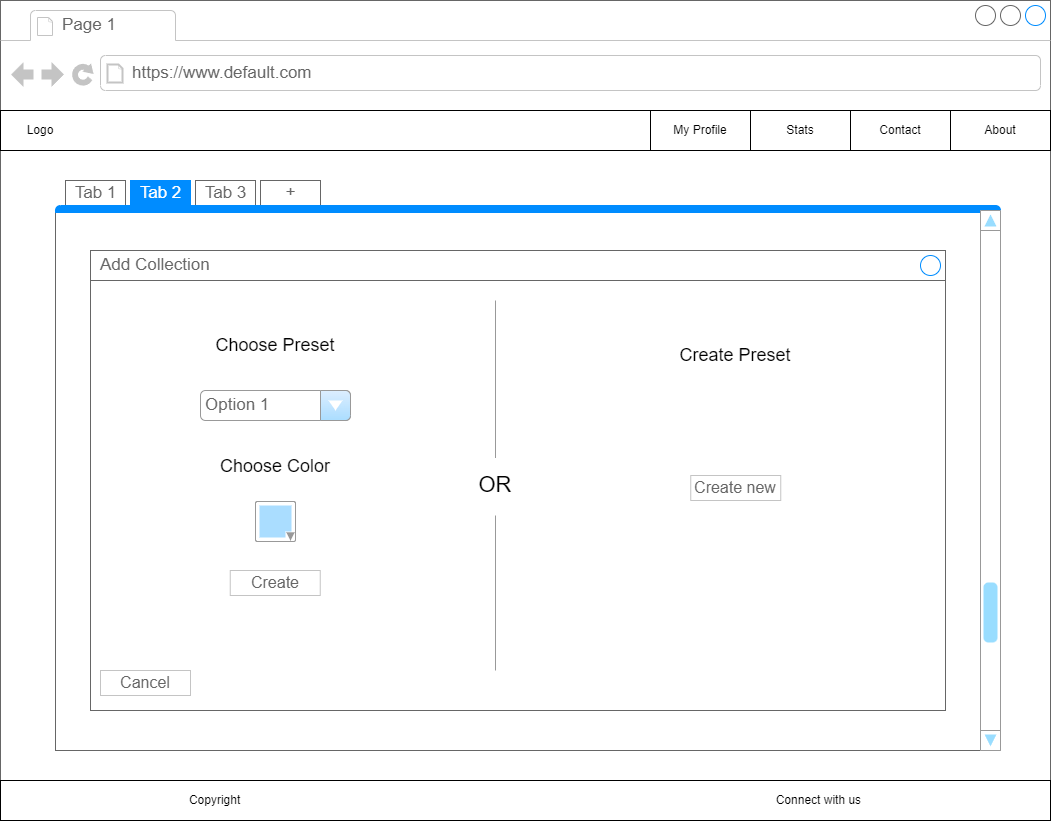
\includegraphics[width=0.6\textwidth]{add_collection_pop_up}
    \caption{'Add Collection' Pop-up}
\end{figure}

\begin{figure}[htbp]
    \centering
    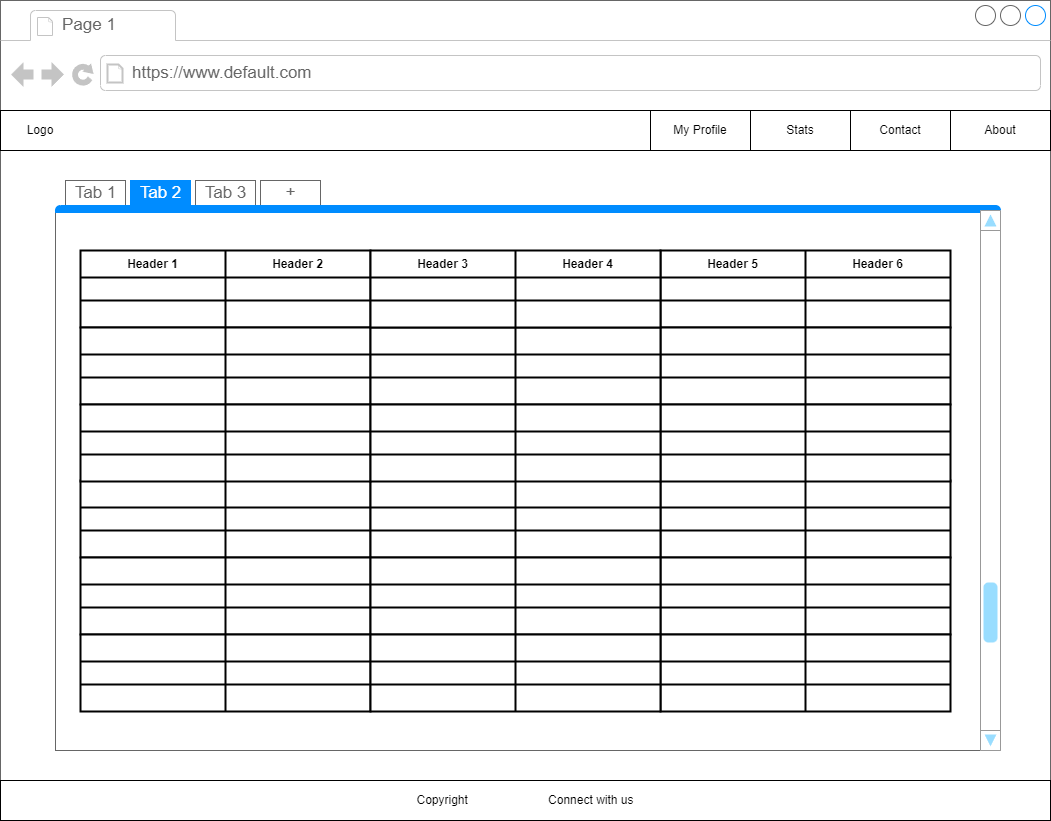
\includegraphics[width=0.6\textwidth]{loggedIn_starting_site}
    \caption{'Logged in' page}
\end{figure}

\begin{figure}[htbp]
    \centering
    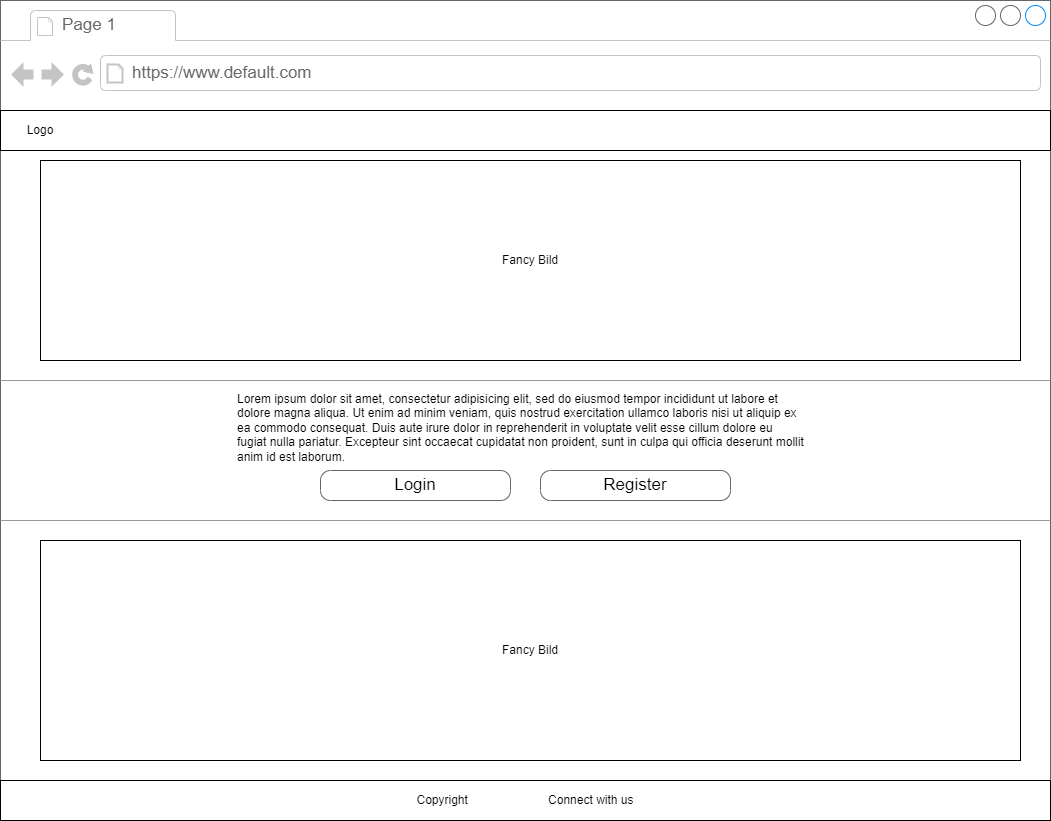
\includegraphics[width=0.6\textwidth]{Starting_site}
    \caption{Starting page}
\end{figure}


\end{document}